\documentclass[11pt]{article}

\usepackage[margin=1in]{geometry}
\usepackage{graphicx}
\usepackage{booktabs}
\usepackage{amsmath, amssymb}
\usepackage{natbib}
\usepackage{hyperref}
\usepackage{xcolor}
\usepackage{caption}
\usepackage{subcaption}
\usepackage{float}
\usepackage{url}
\usepackage{array}

\hypersetup{colorlinks=true, linkcolor=black, citecolor=blue, urlcolor=blue}
\graphicspath{{../output/figures/}}

\title{Who Adopts Buy-Now-Pay-Later, and Why? \\
       \large A Bayesian Hierarchical Re-analysis of a TEP-Based Adoption Survey}
\author{Zan Merrill \and Andy Kim \and Thomas Garner \\[4pt]
        \small OM 386: Advanced Analytics in Marketing \\
        \small McCombs School of Business, The University of Texas at Austin}
\date{Spring 2026}

\begin{document}
\maketitle

\begin{abstract}
\noindent We re-analyze a 226-respondent survey of Buy-Now-Pay-Later (BNPL) adoption
intention originally studied through partial least squares structural
equation modeling \citep{hira2024tep}. Our contribution is a three-stage
pipeline that (i) reduces 28 Likert items to 9 interpretable construct
scores via per-construct PCA, (ii) discovers latent consumer segments
using a finite Gaussian mixture estimated via the EM algorithm, and
(iii) estimates a Bayesian hierarchical linear model of adoption intention
with segment-specific random coefficients via a hand-coded Gibbs sampler.
Three segments emerge from the data, a small group of enthusiasts (17\%),
a larger group of skeptics (39\%), and a moderate majority (44\%), and the
posterior distributions reveal that the drivers of adoption intention
differ sharply across segments: Attitude is the near-deterministic driver
for skeptics, Performance Expectancy and Perceived Usefulness dominate
the moderate segment, and Flexibility emerges as the primary driver for
enthusiasts. The Bayesian posterior lets us state these findings as
explicit probability claims rather than $p$-values.
\end{abstract}

% =============================================================================
\section{Background and Problem}
% =============================================================================

\subsection{Background}

Buy-Now-Pay-Later (BNPL) services have reshaped the short-term consumer
credit market, allowing shoppers to split purchases into smaller, often
interest-free installments at the point of sale. The category is dominated
by Klarna, Afterpay, Affirm, and PayPal Pay in 4, with annual transaction
volume in the United States passing \$100 billion in 2024. Understanding
who adopts BNPL, and why, matters to BNPL providers deciding where to
concentrate acquisition spend, to traditional card issuers considering
entry, and to regulators weighing consumer-protection policy as BNPL
reaches a broader and younger demographic.

\subsection{Data source}

Our analysis uses the 226-respondent survey released with
\citet{hira2024tep}, a recently published paper in the BNPL adoption
literature. The data are secondary: we did not collect them, and all
item wording and construct definitions follow the original paper. The
source PDF is included in the project repository at
\texttt{references/TEP\_BNPL\_paper.pdf}, and the raw response file at
\texttt{data/raw/BNPL Intention to use.xlsx}.

\subsection{Research questions}

Extending this dataset, we ask:
\begin{enumerate}
  \item Can we meaningfully summarize the 28 Likert items as a smaller
        set of interpretable construct scores?
  \item Do distinct consumer segments exist in the data, and how are
        they characterized?
  \item Within each segment, which constructs most drive intention to
        adopt BNPL, and how confident can we be in those drivers?
\end{enumerate}

\subsection{Justification}

\paragraph{Why the question matters.} The original BNPL adoption study
\citep{hira2024tep} estimates one set of coefficients for the entire
226-respondent sample and reports $p$-values as the unit of inference.
That approach answers the question ``what predicts BNPL adoption on
average?'' but leaves a marketing-relevant question unanswered: whether
the \emph{same} factors matter equally for every consumer, or whether
the population decomposes into distinguishable segments whose adoption
is driven by different things. If segments exist and their drivers
differ, messaging and product design should differ by segment as well.

\paragraph{Why these methods.} Three ingredients fit the question.
Per-construct PCA gives principled composite scores without assuming
items are equally informative. Finite Gaussian mixture modeling via EM
(Lecture 13) is the class-taught tool for discovering latent categorical
structure in continuous multivariate data. A Bayesian hierarchical
linear model (Lectures 2 and 3) gives us segment-specific coefficients
with partial pooling across segments, and produces full posterior
distributions rather than point estimates. The Bayesian view is
particularly suited to the small-segment case (Segment 3 has only 38
respondents) because the hyperprior regularizes otherwise high-variance
segment-specific estimates.

\paragraph{What decisions this informs.} The analysis produces
segment-level marketing recommendations, specifically (a) which
construct to emphasize in messaging for each segment, (b) how much
confidence to place in each recommendation given its credible interval
width, and (c) which segments should be prioritized by size versus by
effect strength. Section~4 of this report translates the posterior
findings into specific managerial actions.

% =============================================================================
\section{Data Summary and Exploratory Analysis}
\label{sec:eda}
% =============================================================================

\subsection{Data type and structure}

The data are secondary survey data, with no experimental manipulation.
Each of the 226 respondents answered 28 Likert items on 7-point
agreement scales; no responses are missing. Each item maps to exactly
one of nine theoretical constructs, as defined by \citet{hira2024tep}:
Flexibility (FL, 3 items), Performance Expectancy (PE, 3), Effort
Expectancy (EE, 4), Perceived Autonomy (PA, 3), Perceived Competence
(PC, 3), Perceived Relatedness (PRE, 2), Perceived Usefulness (PU, 3),
Attitude (AT, 4), and Intention to Adopt (IA, 3). Full item wording is
reproduced from the original paper in
\texttt{references/measurement\_items\_table.png}.

\subsection{Item response distributions}

Figure~\ref{fig:item-hist} shows faceted response distributions for all
28 items, colored by parent construct. Responses are moderately
left-skewed for Intention-to-Adopt and Attitude items (most
respondents are positive about BNPL) and closer to symmetric for
Effort Expectancy and Perceived Competence.

\begin{figure}[H]
  \centering
  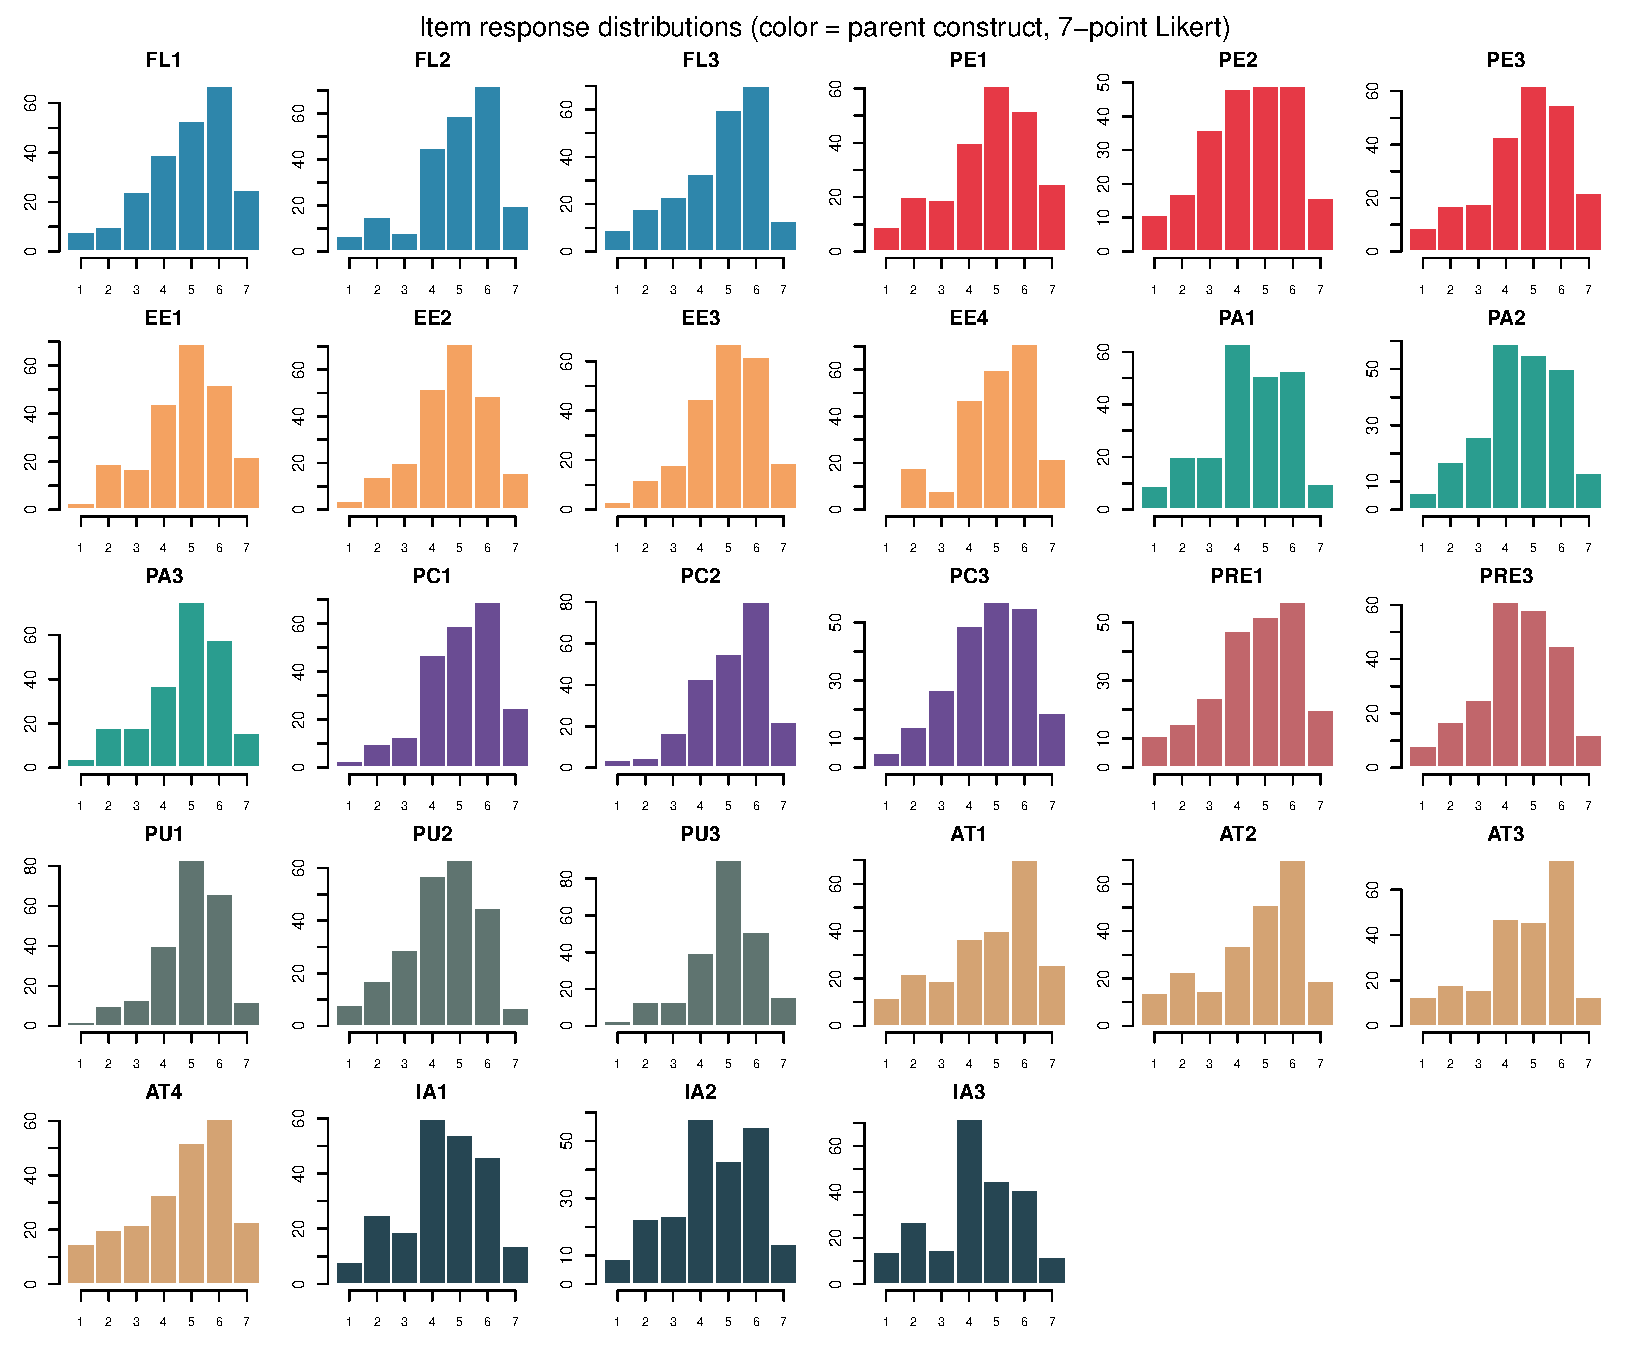
\includegraphics[width=0.95\textwidth]{00_item_response_histograms.pdf}
  \caption{Response distributions for all 28 Likert items, colored by
           parent construct ($N = 226$).}
  \label{fig:item-hist}
\end{figure}

\subsection{Construct-level summary statistics}

After Step 1 (Section~\ref{sec:pca}), each respondent has a score on
each of the nine constructs. Because PC1 is mean-centered and scaled
to unit-variance items, every construct score has mean zero by
construction; the spread is summarized in Table~\ref{tab:sumstats}.

\begin{table}[H]
  \centering
  \caption{Construct-score summary statistics ($N = 226$ respondents).
           All means are zero by construction (PC1 of standardized items).}
  \label{tab:sumstats}
  \begin{tabular}{lcccccc}
    \toprule
    Construct & Items & Mean & SD & Min & Median & Max \\
    \midrule
    Flexibility             & 3 & 0.00 & 1.52 & -4.41 &  0.21 & 2.53 \\
    Performance Expectancy  & 3 & 0.00 & 1.53 & -3.98 &  0.09 & 2.65 \\
    Effort Expectancy       & 4 & 0.00 & 1.66 & -5.24 &  0.24 & 3.17 \\
    Perceived Autonomy      & 3 & 0.00 & 1.53 & -4.29 &  0.11 & 2.92 \\
    Perceived Competence    & 3 & 0.00 & 1.43 & -5.00 &  0.07 & 2.60 \\
    Perceived Relatedness   & 2 & 0.00 & 1.28 & -3.32 &  0.18 & 2.33 \\
    Perceived Usefulness    & 3 & 0.00 & 1.37 & -5.03 & -0.05 & 3.03 \\
    Attitude                & 4 & 0.00 & 1.85 & -4.35 &  0.42 & 2.82 \\
    Intention to Adopt      & 3 & 0.00 & 1.62 & -3.77 & -0.03 & 2.95 \\
    \bottomrule
  \end{tabular}
\end{table}

\subsection{Correlations}

Figure~\ref{fig:corr-heatmap} shows the Pearson correlation matrix of
the nine construct scores. Every pairwise correlation is positive,
consistent with a single ``positive BNPL disposition'' latent direction
running through much of the data, but the correlations are not so
extreme that the constructs collapse to a single factor. Attitude is
most strongly correlated with Intention to Adopt ($r = 0.75$),
consistent with Attitude's role in the theory as a proximal antecedent
to behavior. Perceived Competence correlates most weakly with the rest
of the set.

\begin{figure}[H]
  \centering
  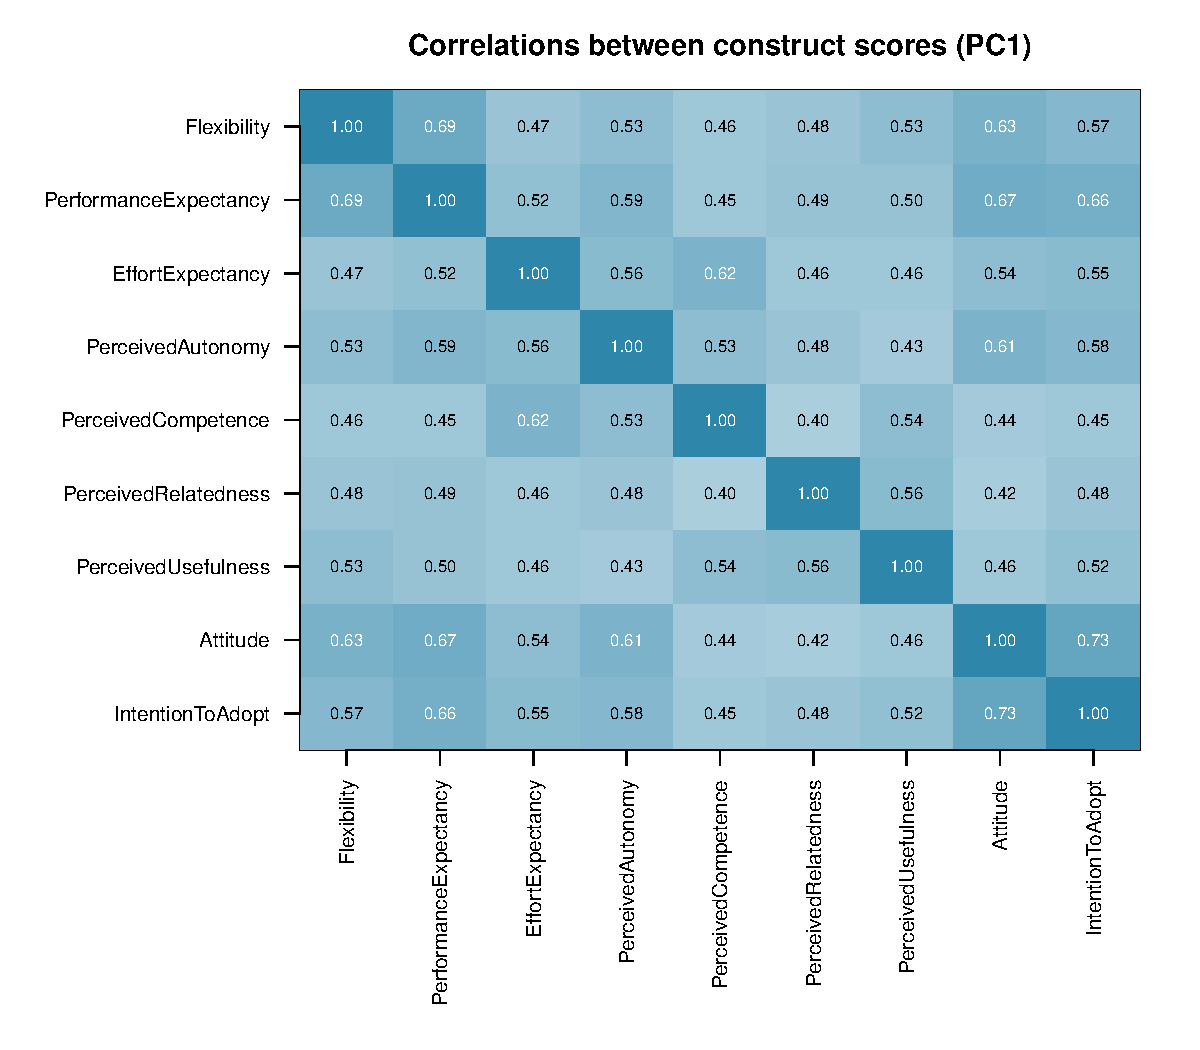
\includegraphics[width=0.72\textwidth]{00_construct_correlation_heatmap.pdf}
  \caption{Pearson correlations between the nine construct scores
           (PC1 per construct).}
  \label{fig:corr-heatmap}
\end{figure}

\subsection{Baseline regression}

Before modeling heterogeneity, we fit a single complete-pooling OLS
regression of Intention to Adopt on the eight predictor scores as an
exploratory baseline (Table~\ref{tab:ols-baseline}). Three predictors
are statistically significant at conventional levels: Attitude
($\beta = 0.39$, $p < 0.001$), Performance Expectancy
($\beta = 0.20$, $p = 0.005$), and Perceived Usefulness
($\beta = 0.15$, $p = 0.024$). The model explains 62.5\% of the
variance in Intention to Adopt ($R^2 = 0.625$,
$\text{adj.}\,R^2 = 0.612$), which sets a useful benchmark for the
hierarchical model in Section~\ref{sec:hlm}.

\begin{table}[H]
  \centering
  \caption{Complete-pooling OLS regression: Intention to Adopt on the
           eight predictor construct scores.}
  \label{tab:ols-baseline}
  \begin{tabular}{lccc}
    \toprule
    Predictor                  & Estimate & SE    & $p$-value \\
    \midrule
    (Intercept)                &  0.000   & 0.067 & 1.000 \\
    Flexibility                & -0.022   & 0.068 & 0.741 \\
    Performance Expectancy     &  0.200   & 0.071 & 0.005 \\
    Effort Expectancy          &  0.094   & 0.059 & 0.111 \\
    Perceived Autonomy         &  0.083   & 0.063 & 0.192 \\
    Perceived Competence       & -0.022   & 0.067 & 0.743 \\
    Perceived Relatedness      &  0.093   & 0.069 & 0.180 \\
    Perceived Usefulness       &  0.155   & 0.068 & 0.024 \\
    Attitude                   &  0.385   & 0.055 & $<0.001$ \\
    \midrule
    \multicolumn{4}{l}{$R^2 = 0.625$, $\text{adj.}\,R^2 = 0.612$,
                       residual SE $= 1.012$ on 217 df, $N = 226$} \\
    \bottomrule
  \end{tabular}
\end{table}

Pairwise scatterplots of all constructs appear in Figure~\ref{fig:pairs}
in the appendix.

% =============================================================================
\section{Data Analyses, Key Findings, and Conclusions}
\label{sec:analyses}
% =============================================================================

Our analysis proceeds in three stages: dimensionality reduction
(Section~\ref{sec:pca}), model-based segmentation
(Section~\ref{sec:cluster}), and Bayesian hierarchical regression
(Section~\ref{sec:hlm}). Each stage uses a class-taught technique
(PCA, finite-mixture EM from Lecture 13, and Bayesian hierarchical
modeling from Lectures 2 and 3).

% -----------------------------------------------------------------------------
\subsection{Step 1: Construct scores via PCA}
\label{sec:pca}
% -----------------------------------------------------------------------------

\paragraph{Why PCA per construct.} Standard practice in the TEP and
UTAUT survey traditions is to average the items in each construct
with equal weights. This implicitly assumes every item is equally
informative about the latent construct. We relax that assumption by
running PCA on each construct's items separately and using the first
principal component (PC1) as the score, so items are weighted by how
much they contribute to shared variance. This follows the Lecture 1
framing of PCA as an exploratory dimensionality-reduction tool.

\paragraph{Procedure.} For each of the nine constructs, we
(i) standardize the items, (ii) run \texttt{prcomp} on the correlation
matrix, and (iii) flip the sign of PC1 if needed so that higher scores
correspond to the ``high construct'' direction. Each respondent's
score on construct $c$ is then the value of their PC1 for construct
$c$.

\paragraph{Result.} Figure~\ref{fig:pca-varexp} shows the proportion
of variance explained by PC1 for each construct. Every construct has
PC1 variance explained at least 0.63; six of nine exceed 0.75. The
lowest is Perceived Usefulness (0.63), still well above the 0.5
threshold for justifying a single-component summary. We carry forward
the 9-column matrix of PC1 scores as input to the next stage.

\begin{figure}[H]
  \centering
  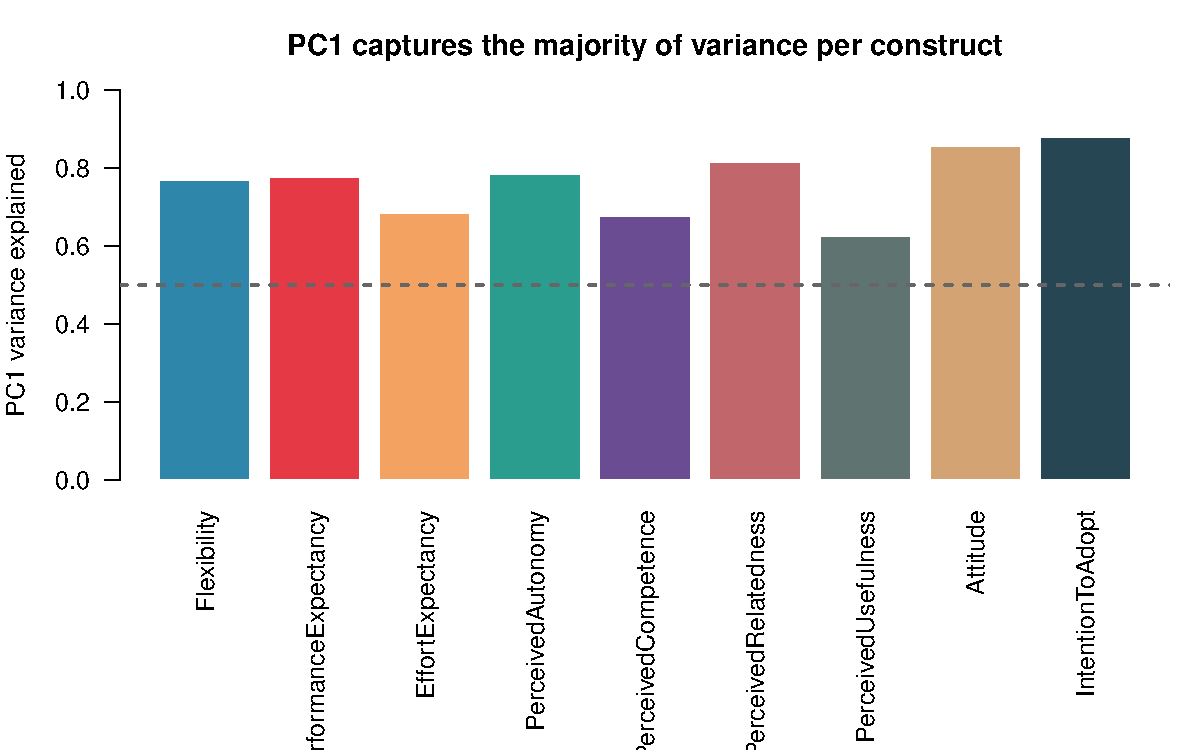
\includegraphics[width=0.72\textwidth]{01_pca_variance_explained.pdf}
  \caption{PC1 variance explained per construct. The dashed line
           marks the 0.5 threshold. Colors are retained as a
           consistent per-construct palette throughout the report.}
  \label{fig:pca-varexp}
\end{figure}

% -----------------------------------------------------------------------------
\subsection{Step 2: Discovering consumer segments}
\label{sec:cluster}
% -----------------------------------------------------------------------------

\paragraph{Why a finite mixture.} We want to discover \emph{latent}
segments: there is no label in the data telling us who belongs to
which group. Finite Gaussian mixture models, estimated via the EM
algorithm \citep{dempster1977em}, are the canonical tool for exactly
this problem and are the segmentation method taught in OM 386
Lecture 13. The model places each respondent's predictor vector in
one of $K$ multivariate normal components, with component means,
covariances, and mixing proportions jointly estimated from the data.

\paragraph{Setup.} We use the eight predictor construct scores,
standardized to unit variance, as the input to the mixture. The
outcome Intention to Adopt is held out for Step 3. We estimate two
implementations of the same model.

\begin{enumerate}
  \item \texttt{mclust::Mclust} \citep{fraley2002mclust}, which
        searches over $K \in \{1, \dots, 9\}$ and the 14 possible
        covariance parameterizations, selecting the combination with
        the best Bayesian Information Criterion \citep{schwarz1978bic}.
  \item A hand-coded EM sampler that directly generalizes the
        Lecture 13 regression-mixture code from a one-dimensional
        regression mixture to $p$-dimensional unsupervised
        clustering. Log-sum-exp is used in the E-step for numerical
        stability; full covariance matrices in each component; a
        convergence tolerance of $10^{-8}$ on the log-likelihood.
\end{enumerate}

\paragraph{Result: three segments.} The BIC search over $K$ and
covariance structure is shown in Figure~\ref{fig:mclust-bic}; the
optimum is $K = 3$. The hand-coded EM sampler, initialized from
$k$-means seeds and run at $K = 3$, converges in 85 iterations
(Figure~\ref{fig:handem}). The two implementations agree on $K = 3$
and on the qualitative character of the three segments. Segment
membership agrees moderately well (adjusted Rand index of 0.55),
with the differences mostly concentrated along the boundary between
the two larger groups.

\begin{figure}[H]
\centering
\begin{subfigure}{0.48\textwidth}
  \centering
  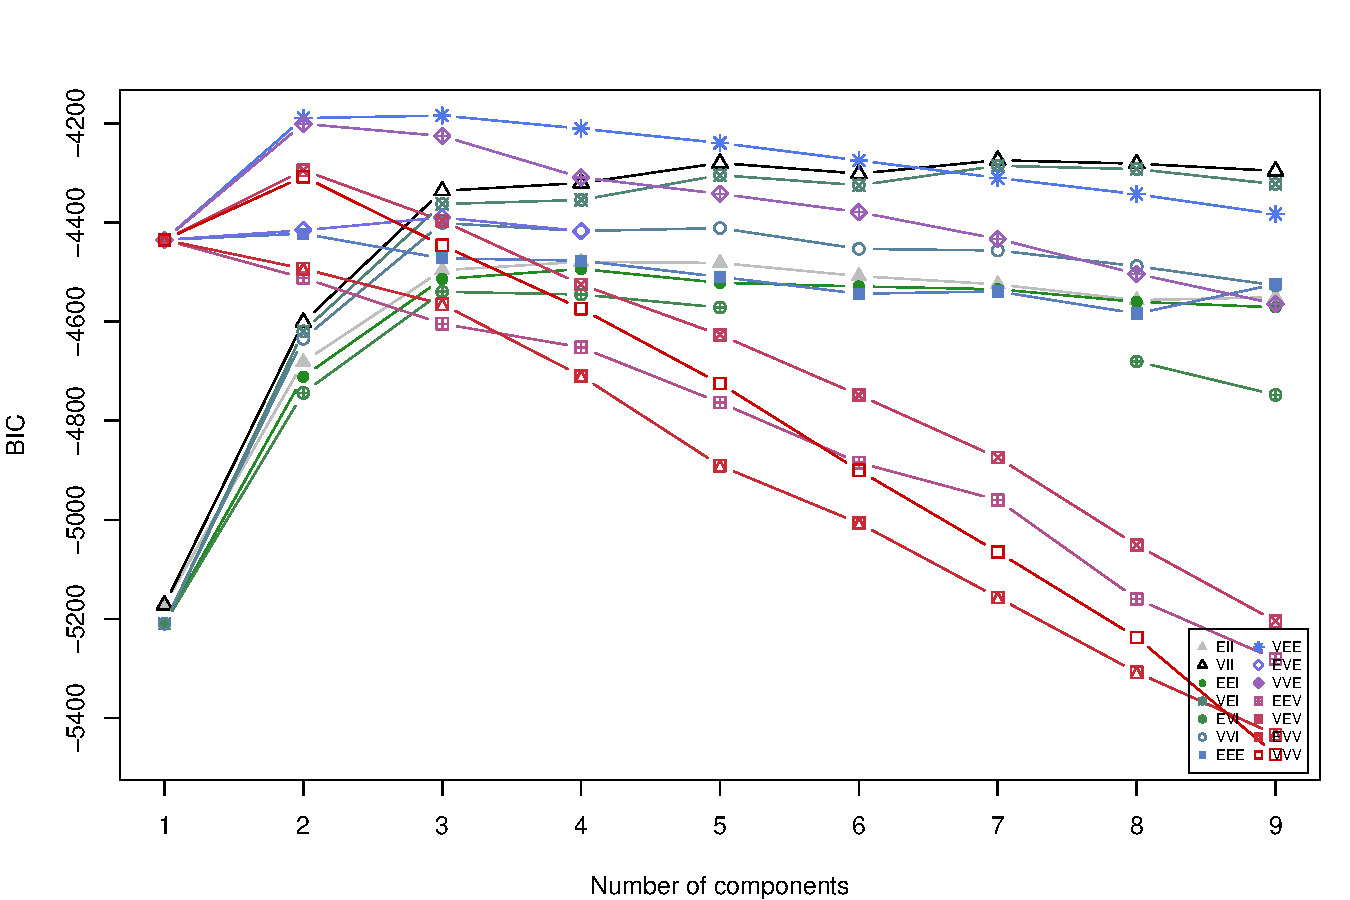
\includegraphics[width=\linewidth]{02_mclust_bic.pdf}
  \caption{\texttt{mclust} BIC search. The peak, which the BIC
           convention places at the maximum, is at $K = 3$.}
  \label{fig:mclust-bic}
\end{subfigure}\hfill
\begin{subfigure}{0.48\textwidth}
  \centering
  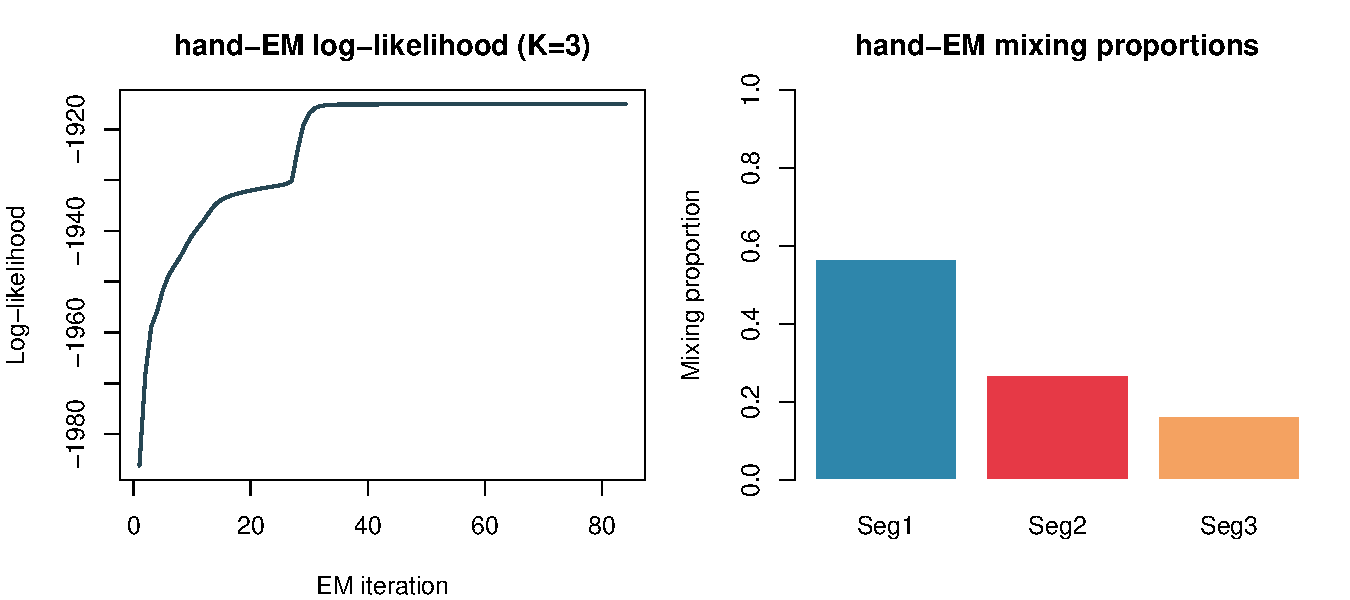
\includegraphics[width=\linewidth]{02_handem_diagnostics.pdf}
  \caption{Hand-coded EM log-likelihood trace (left) and converged
           mixing proportions (right) at $K = 3$.}
  \label{fig:handem}
\end{subfigure}
\caption{Two implementations of the Lecture 13 finite-mixture model
         on the eight predictor construct scores.}
\end{figure}

\paragraph{Segment profiles.} Figure~\ref{fig:profiles} shows the
mean standardized construct score for each predictor, by segment, for
the winning \texttt{mclust} solution. The interpretation is immediate:

\begin{itemize}
  \item Segment 1 (``Moderates,'' $n = 99$, 44\% of the sample) is
        near zero on every predictor. This is the neutral majority:
        mildly positive Attitude, otherwise close to the sample mean
        on every construct.
  \item Segment 2 (``Skeptics,'' $n = 89$, 39\%) is negative on all
        eight predictors. Attitude toward BNPL is the most negative
        (mean $-0.66$ standard deviations), and these respondents
        broadly distrust the product category.
  \item Segment 3 (``Enthusiasts,'' $n = 38$, 17\%) is highly
        positive on every predictor (means 0.8 to 1.1). They see
        BNPL as useful, flexible, autonomous, and connected.
\end{itemize}

\begin{figure}[H]
  \centering
  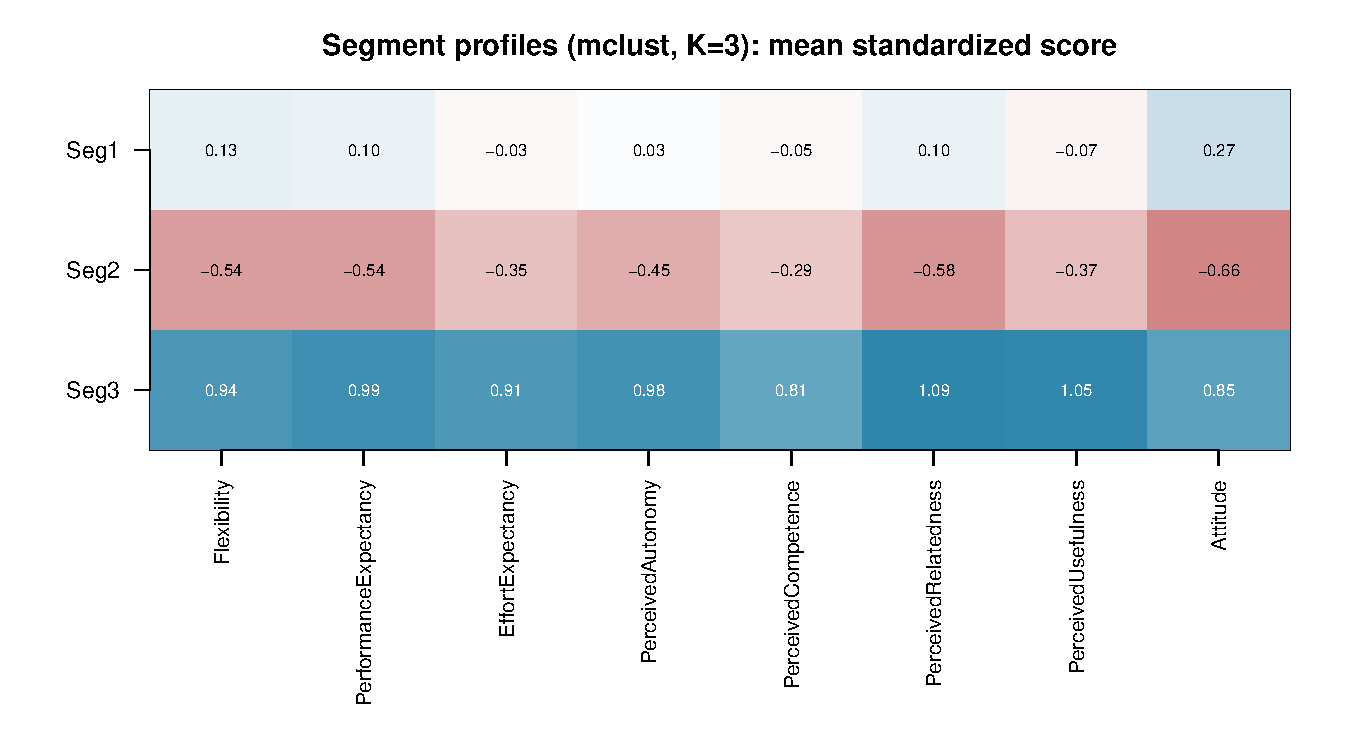
\includegraphics[width=0.9\textwidth]{02_segment_profiles_winner.pdf}
  \caption{Segment profiles from the winning \texttt{mclust}
           solution: mean standardized construct score per predictor
           per segment. Blue values are above the sample average,
           red below.}
  \label{fig:profiles}
\end{figure}

We carry the \texttt{mclust} labels forward to Step 3 because
\texttt{mclust} picks the best covariance structure automatically
via BIC, whereas the hand-coded EM is hard-wired to full
covariance. The two segmentations agree on the number and broad
character of the segments; downstream conclusions are robust to
this choice.

% -----------------------------------------------------------------------------
\subsection{Step 3: Bayesian hierarchical linear model}
\label{sec:hlm}
% -----------------------------------------------------------------------------

\paragraph{Goal.} Within each segment, quantify the posterior
distribution of each predictor's effect on Intention to Adopt.

\paragraph{Model.} Let $y_i$ denote respondent $i$'s Intention-to-Adopt
score, $\mathbf{x}_i \in \mathbb{R}^{9}$ the vector of eight predictor
scores with an intercept, and $s_i \in \{1, 2, 3\}$ the segment
assignment from Section~\ref{sec:cluster}. Our model is:
\begin{align}
  y_i                      &\sim \mathcal{N}(\mathbf{x}_i' \boldsymbol{\beta}_{s_i},\; \tau^{-1}), \\
  \boldsymbol{\beta}_k      &\sim \mathcal{N}(\boldsymbol{\mu}_\beta,\; \boldsymbol{\Sigma}_\beta),
                              \quad k = 1, 2, 3, \\
  \boldsymbol{\mu}_\beta    &\sim \mathcal{N}(\mathbf{0},\; 10^6 \mathbf{I}_9)
                              \qquad \text{(diffuse hyperprior)}, \\
  \boldsymbol{\Sigma}_\beta &\sim \mathcal{IW}(11,\; \mathbf{I}_9)
                              \qquad \text{(weakly informative)}, \\
  \tau                     &\sim \text{Gamma}(\tfrac{1}{2},\; \tfrac{1}{2}).
\end{align}
The hierarchical structure partially pools information across
segments: segments with more respondents (Segments 1 and 2) get
sharper posteriors driven by their own data, while the small
Segment 3 ($n = 38$) borrows strength from the overall mean.

\paragraph{Estimation.} We implement a Gibbs sampler by extending the
Normal-Gamma conjugate template from Lecture 3 (see
\texttt{data\_examples/BayeianLM.r}) to the hierarchical structure
above. All four full conditionals are conjugate: per-segment
$\boldsymbol{\beta}_k$ is multivariate normal,
$\boldsymbol{\mu}_\beta$ is multivariate normal,
$\boldsymbol{\Sigma}_\beta$ is Inverse-Wishart, and $\tau$ is Gamma.
We run 10{,}000 post-burn-in iterations (with 2{,}000 burn-in), warm-
starting from segment-stratified OLS estimates. The sampler completes
in under 6 seconds of wall time.

\paragraph{Chain diagnostics.} Figure~\ref{fig:trace} shows trace
plots for the segment intercepts and for the Attitude slope. Chains
mix rapidly with no visible drift, indicating convergence. The
residual precision $\tau$ and the induced residual standard deviation
$\sqrt{1/\tau}$ also mix well (Figure~\ref{fig:trace-tau} in the
appendix); the posterior-mean residual SD is 1.02, with 90\%
credible interval $[0.94, 1.10]$. This is close to the residual SE
of 1.01 from the baseline OLS in Section~\ref{sec:eda}, a useful
sanity check that the sampler is anchored correctly.

\begin{figure}[H]
  \centering
  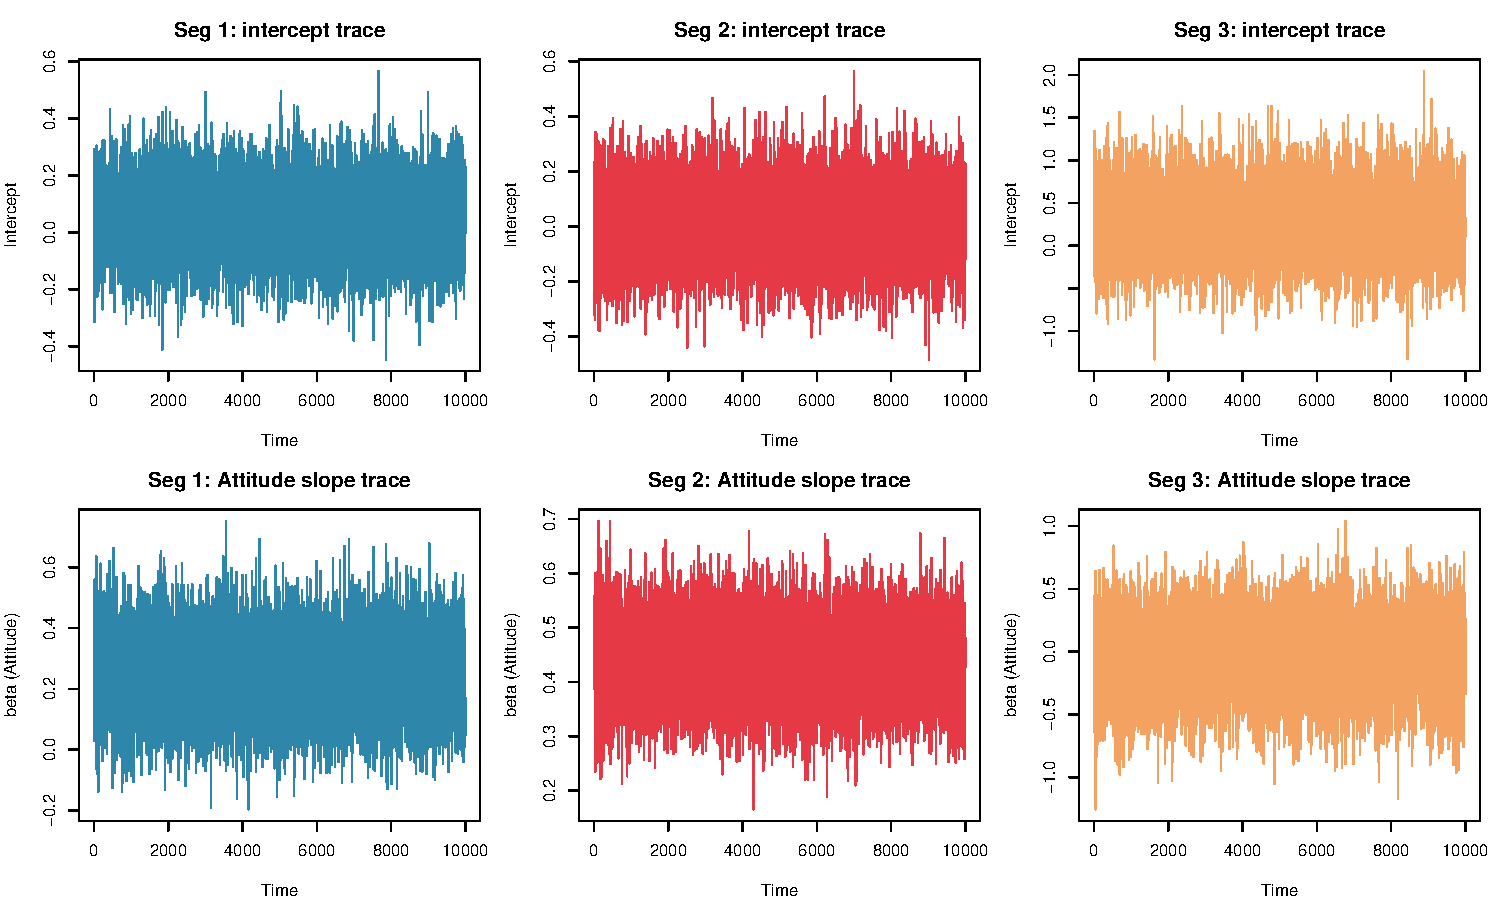
\includegraphics[width=0.95\textwidth]{03_trace_plots.pdf}
  \caption{Trace plots for segment intercepts (top row) and for the
           Attitude slope (bottom row), colored by segment. Chains
           are well-mixed with no visible drift.}
  \label{fig:trace}
\end{figure}

\paragraph{Key result: drivers differ across segments.}
Figure~\ref{fig:forest} and Figure~\ref{fig:densities} show the
per-segment posterior coefficients. The pattern is striking.

\begin{itemize}
  \item Segment 1 (Moderates). Adoption intention is driven by
        Performance Expectancy
        ($\bar{\beta} = 0.28$, $P(\beta > 0) = 0.97$),
        Perceived Usefulness
        ($\bar{\beta} = 0.28$, $P(\beta > 0) = 0.98$), and
        Attitude ($\bar{\beta} = 0.25$, $P(\beta > 0) = 0.98$).
        Rational and evaluative drivers dominate.
  \item Segment 2 (Skeptics). Attitude is the near-deterministic
        driver ($\bar{\beta} = 0.44$, $P(\beta > 0) = 1.00$).
        Performance Expectancy
        ($\bar{\beta} = 0.18$, $P(\beta > 0) = 0.99$) and
        Perceived Usefulness
        ($\bar{\beta} = 0.13$, $P(\beta > 0) = 0.94$) contribute
        secondarily. Shifting the affective orientation of this
        group is the single largest lever in the entire analysis.
  \item Segment 3 (Enthusiasts). Flexibility emerges as the
        strongest driver ($\bar{\beta} = 0.40$,
        $P(\beta > 0) = 0.92$). Posteriors are wider for this
        segment because it contains only 38 respondents, so claims
        about Segment 3 should be held more loosely.
\end{itemize}

\begin{figure}[H]
  \centering
  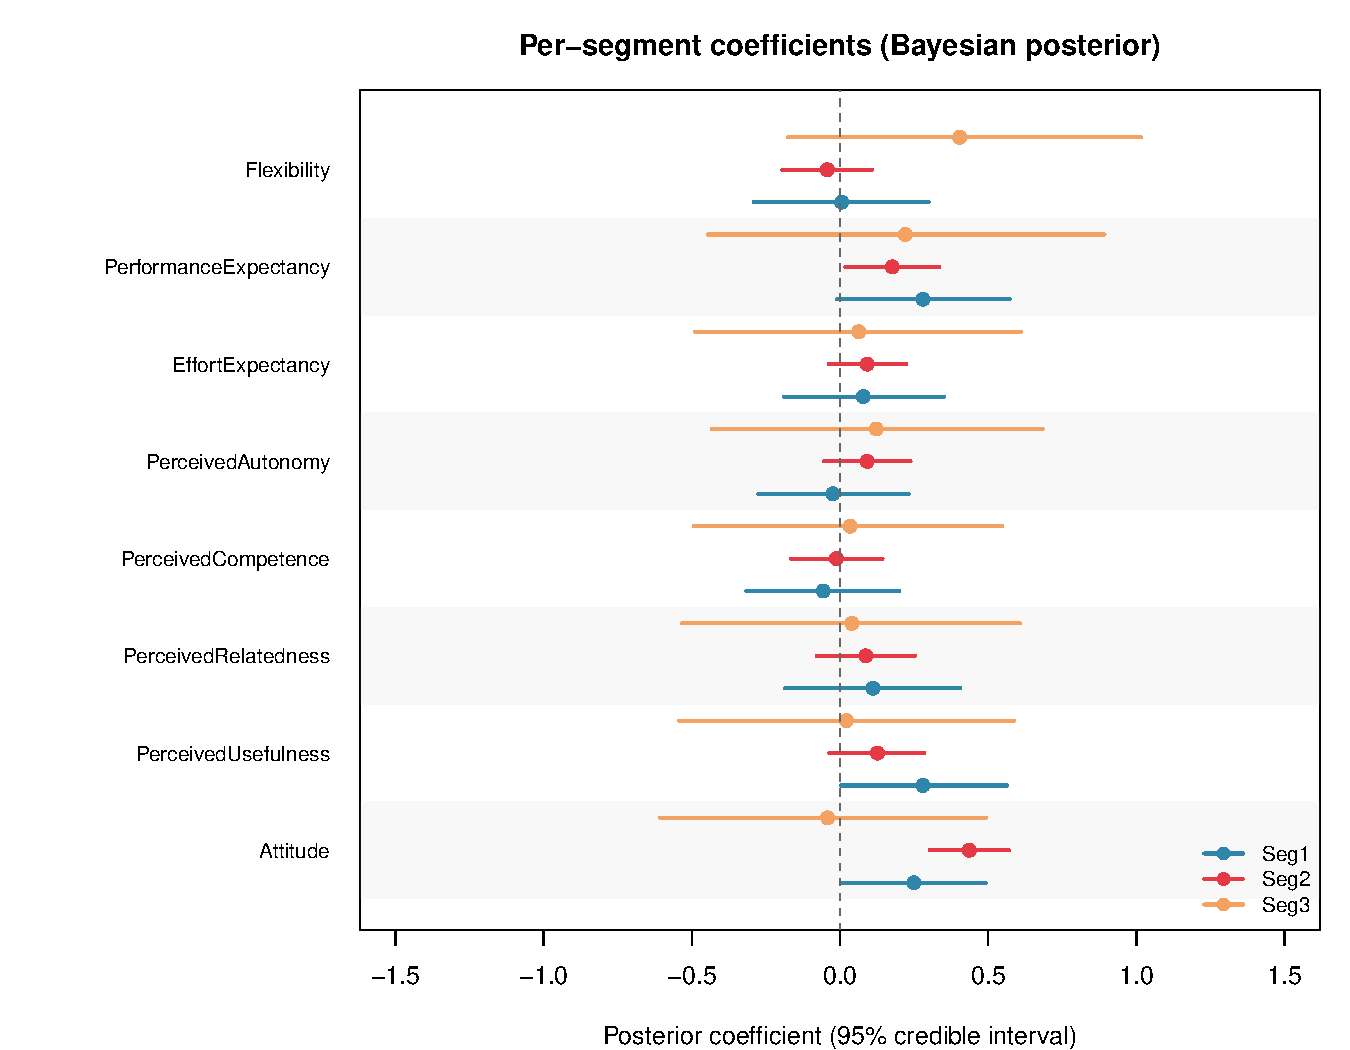
\includegraphics[width=0.85\textwidth]{03_forest_by_segment.pdf}
  \caption{Per-segment posterior coefficients with 90\% credible
           intervals (intercept omitted). Dots are posterior means;
           bars are 90\% credible intervals. Colors denote segment.}
  \label{fig:forest}
\end{figure}

\begin{figure}[H]
  \centering
  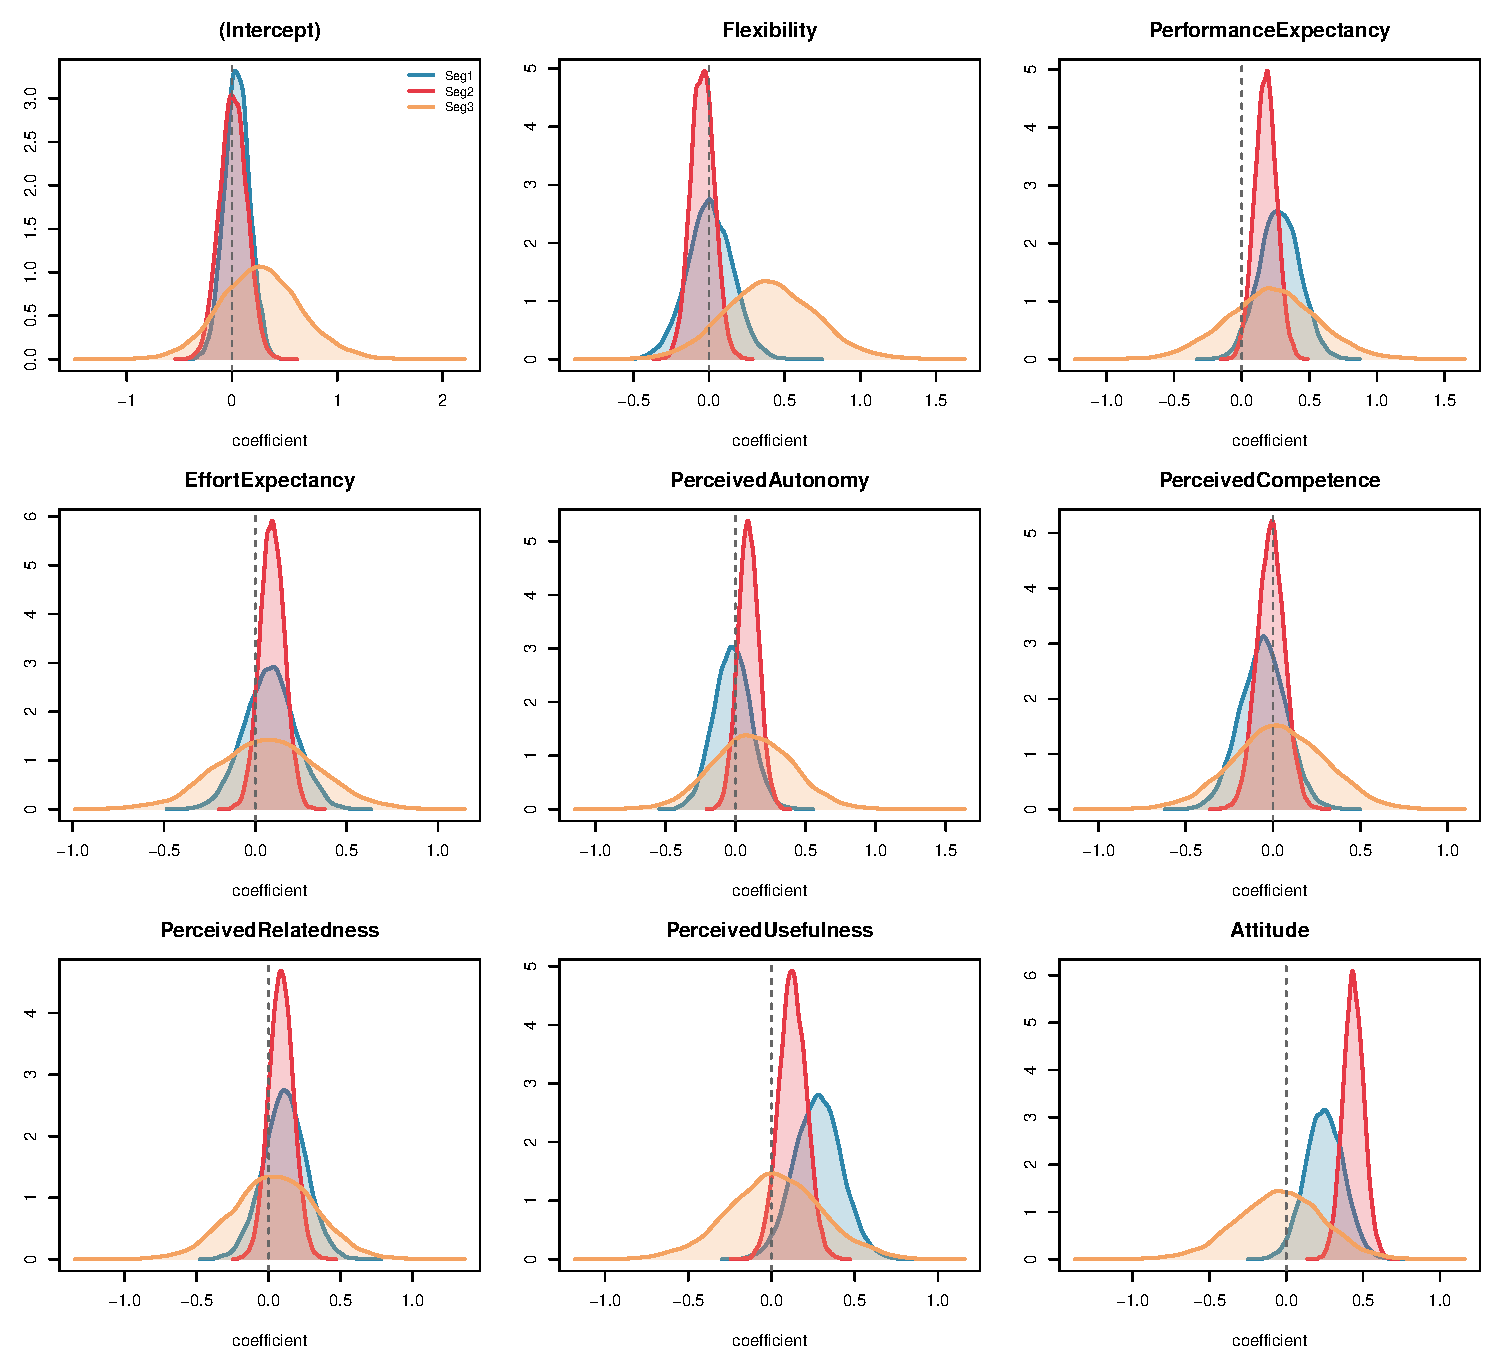
\includegraphics[width=0.95\textwidth]{03_posterior_densities.pdf}
  \caption{Posterior densities of each coefficient by segment.
           Vertical dashed line is zero. Colored shading is each
           segment's posterior; distinct shapes across segments are
           the core heterogeneity finding.}
  \label{fig:densities}
\end{figure}

\paragraph{Sanity checks.} We cross-validate the Bayesian posterior
against two alternatives: a complete-pooling OLS fit (one $\boldsymbol{\beta}$
for all 226 respondents) and a random-intercept fit in
\texttt{lme4::lmer}. The posterior-mean hyper-coefficients
$\boldsymbol{\mu}_\beta$ line up with the \texttt{lmer} fixed
effects, with the largest discrepancy on Attitude (0.17 units,
reflecting the Bayesian model's allowance for segment-specific
slopes). The \texttt{lmer} fit also triggers a boundary-singular-fit
warning, indicating that once segment-specific slopes are allowed,
there is very little residual between-segment variance in the
\emph{intercept}. This is itself an important finding: segments
differ in their \emph{slopes}, not their baseline intention.
Figure~\ref{fig:shrinkage} illustrates the shrinkage signature of
partial pooling for the Attitude slope; each segment's Bayesian
posterior mean sits between its no-pool OLS estimate and the
complete-pool estimate.

\begin{figure}[H]
  \centering
  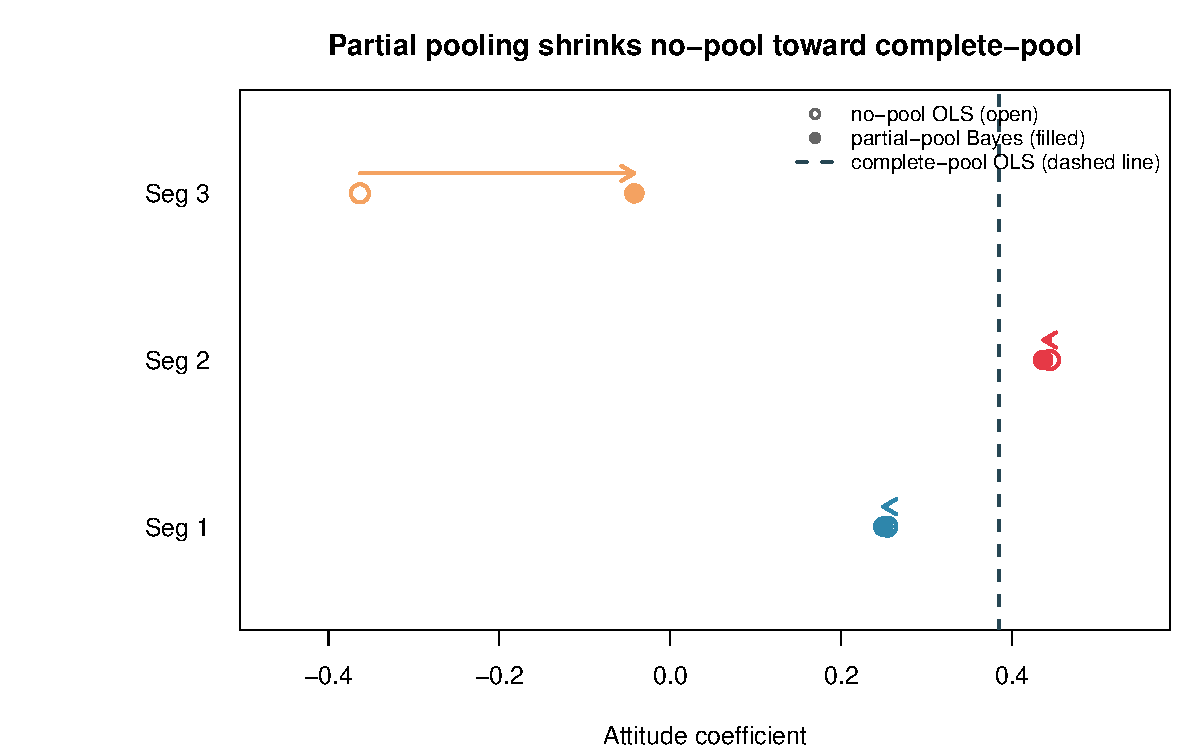
\includegraphics[width=0.72\textwidth]{03_shrinkage_illustration.pdf}
  \caption{Partial-pooling shrinkage for the Attitude slope. Open
           circles are segment-stratified OLS estimates (no pooling);
           filled circles are Bayesian posterior means (partial
           pooling); the dashed vertical line is the complete-pooling
           OLS estimate.}
  \label{fig:shrinkage}
\end{figure}

% =============================================================================
\section{Recommendations, Limitations, and Future Research}
% =============================================================================

\subsection{Managerial recommendations}

The three segments require three different marketing playbooks.

\begin{itemize}
  \item Reach the Skeptics through affect, not features. Because
        Attitude is the near-deterministic driver for Segment 2
        ($P(\beta > 0) = 1.00$), campaigns aimed at this group should
        prioritize how BNPL \emph{feels} (trust, simplicity, peace of
        mind) over feature-by-feature comparison with credit cards.
        This is the largest high-probability effect in the analysis,
        and the Skeptics are 39\% of the sample, so the expected
        uplift from moving them is substantial.
  \item Sell Moderates on utility. For the neutral majority, both
        Performance Expectancy and Perceived Usefulness matter
        roughly equally and credibly. Concrete use-case messaging
        (``split a \$200 purchase into four zero-interest payments'')
        maps directly to what this segment weighs.
  \item Sell Enthusiasts on flexibility. The already-positive
        Enthusiast segment is primarily driven by Flexibility.
        Messaging around control, customization, and choice of
        repayment schedule should move them further. Because this
        segment is smaller, however, acquisition spend should be
        sized accordingly.
  \item Prioritize by segment size and effect strength. Segment 2
        (Skeptics) combines the largest high-probability effect
        (Attitude, $P(\beta > 0) = 1.00$) with 39\% of the sample,
        making it the highest expected-value marketing target.
        Segment 1 (Moderates) is the largest group at 44\% with
        moderate effect sizes. Segment 3 (Enthusiasts) is a smaller,
        easier-to-close audience.
\end{itemize}

\subsection{Limitations}

\begin{enumerate}
  \item Sample size. $N = 226$ is adequate for the aggregate
        regression but leaves Segment 3 ($n = 38$) with visibly
        wider credible intervals. Claims about this segment should
        be held more loosely than the Seg 1 and Seg 2 findings.
  \item Cross-sectional survey data. The outcome is self-reported
        \emph{intention}, not observed adoption behavior. The
        intention-to-behavior gap is well documented in technology
        adoption research.
  \item Singular-fit warning in \texttt{lme4}. The random-intercept
        validation produced a boundary-singular fit (between-segment
        intercept variance estimated at zero). The Bayesian model
        handles this gracefully via the hyperprior on
        $\boldsymbol{\mu}_\beta$, but it confirms that the
        interesting heterogeneity is in slopes, not intercepts.
  \item Self-reported Likert data. Construct scores inherit all the
        usual weaknesses of self-report (social desirability, common
        method bias, response style). PCA cleaning does not address
        these.
  \item Segment identification is conditional. We treat the Step 2
        segment labels as fixed inputs to Step 3. A more principled
        approach would propagate segment-membership uncertainty into
        the posterior coefficients (see future research below).
\end{enumerate}

\subsection{Future research}

Three natural extensions follow directly from this work. First, a
longitudinal replication with actual BNPL adoption behavior as the
outcome (rather than self-reported intention) would strengthen the
causal interpretation of the segment-level drivers. Second, within the
present data, a joint latent-class regression model estimated by EM
would merge Steps 2 and 3 into a single procedure and propagate
segment-membership uncertainty directly into the coefficient
posteriors. Third, adding demographic and behavioral covariates (age,
income, prior credit-card use, shopping frequency) to the segmentation
step would let us describe \emph{who} the Skeptics, Moderates, and
Enthusiasts actually are, which is the immediate next question a BNPL
marketer would ask.

% =============================================================================
\bibliographystyle{plainnat}
\bibliography{references}

% =============================================================================
\appendix
\section*{Appendix}
% =============================================================================

\subsection*{A. Measurement items} \label{appendix:items}
The full item wording is reproduced from \citet{hira2024tep}
Table A1, available as
\texttt{references/measurement\_items\_table.png} in the repository.

\subsection*{B. Pairwise construct-score scatterplots}
\begin{figure}[H]
  \centering
  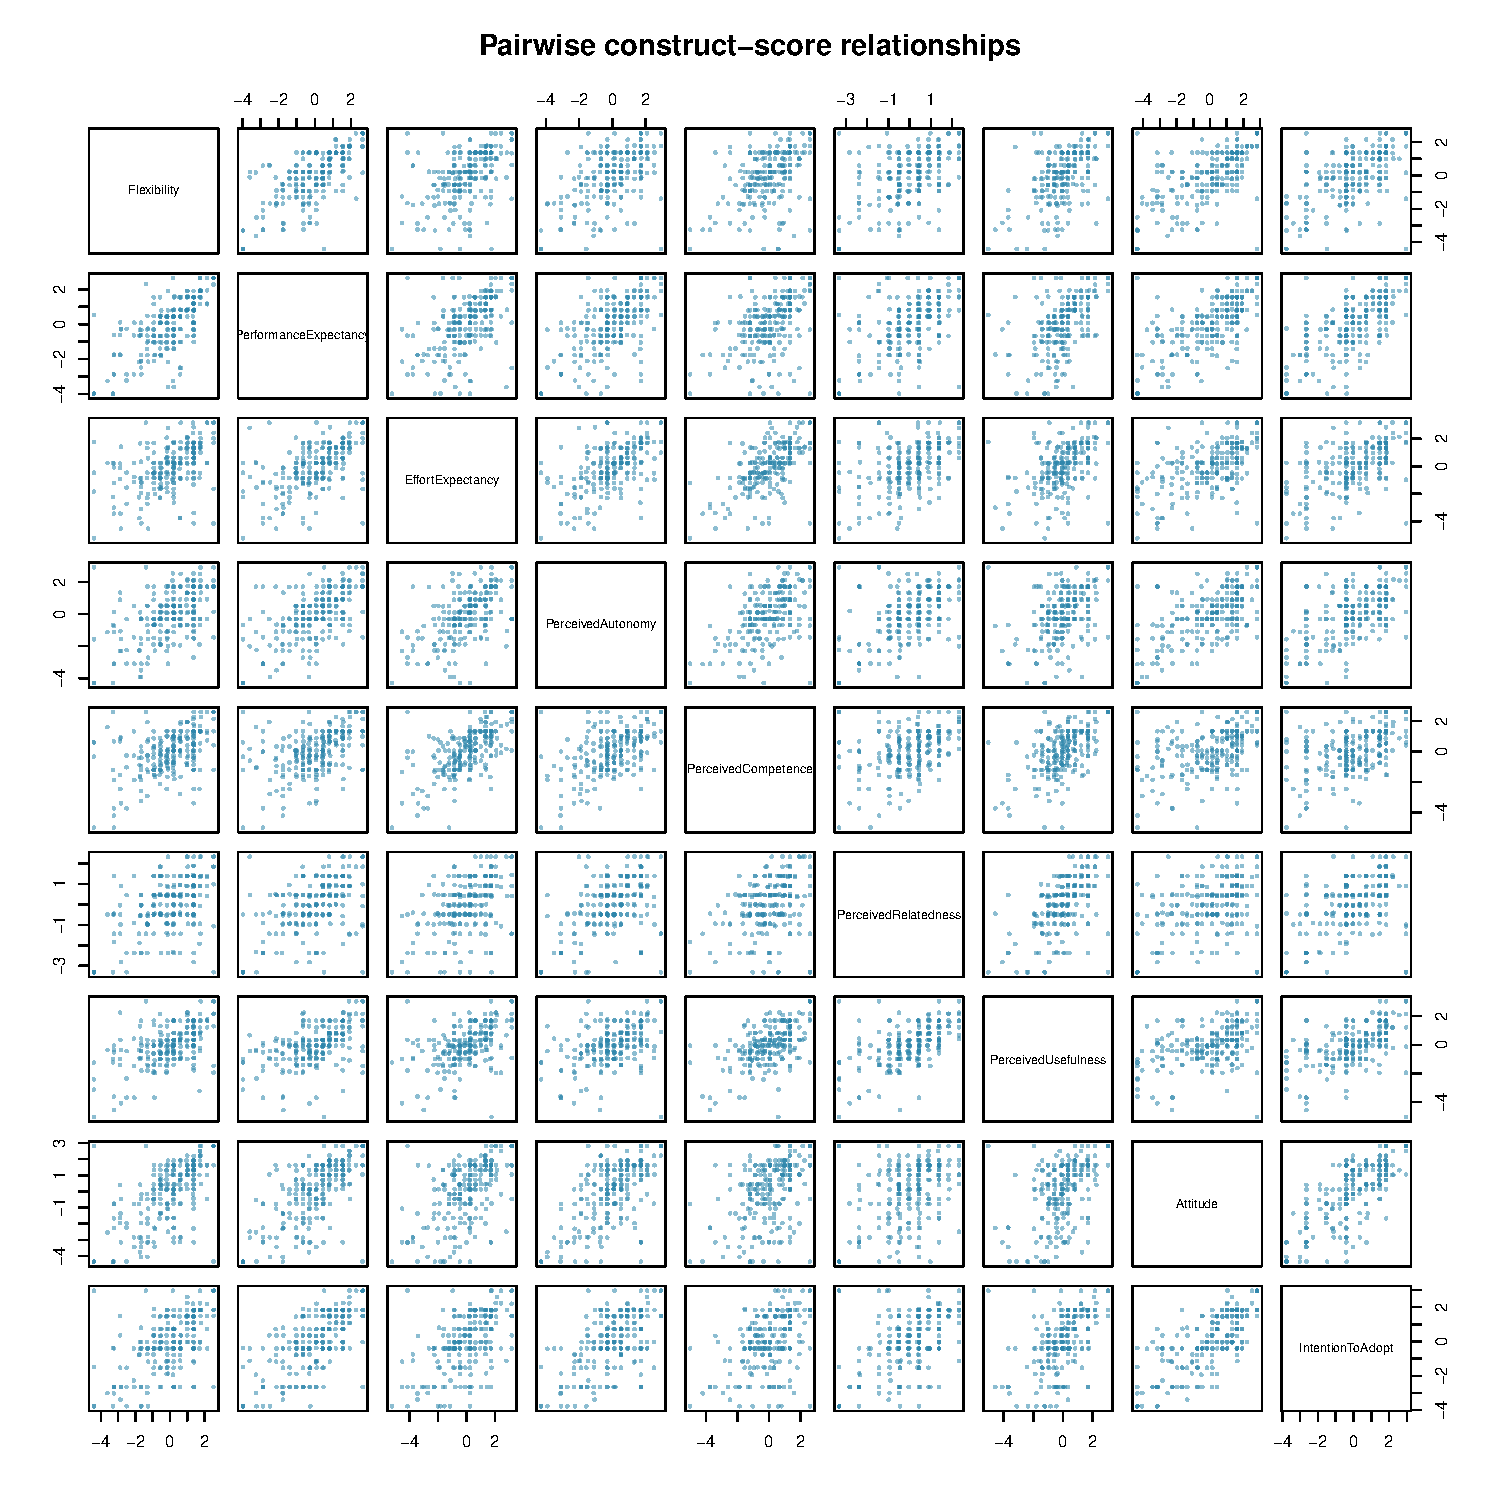
\includegraphics[width=0.9\textwidth]{00_construct_pairs.pdf}
  \caption{Pairwise construct-score scatterplots.}
  \label{fig:pairs}
\end{figure}

\subsection*{C. Residual-precision trace}
\begin{figure}[H]
  \centering
  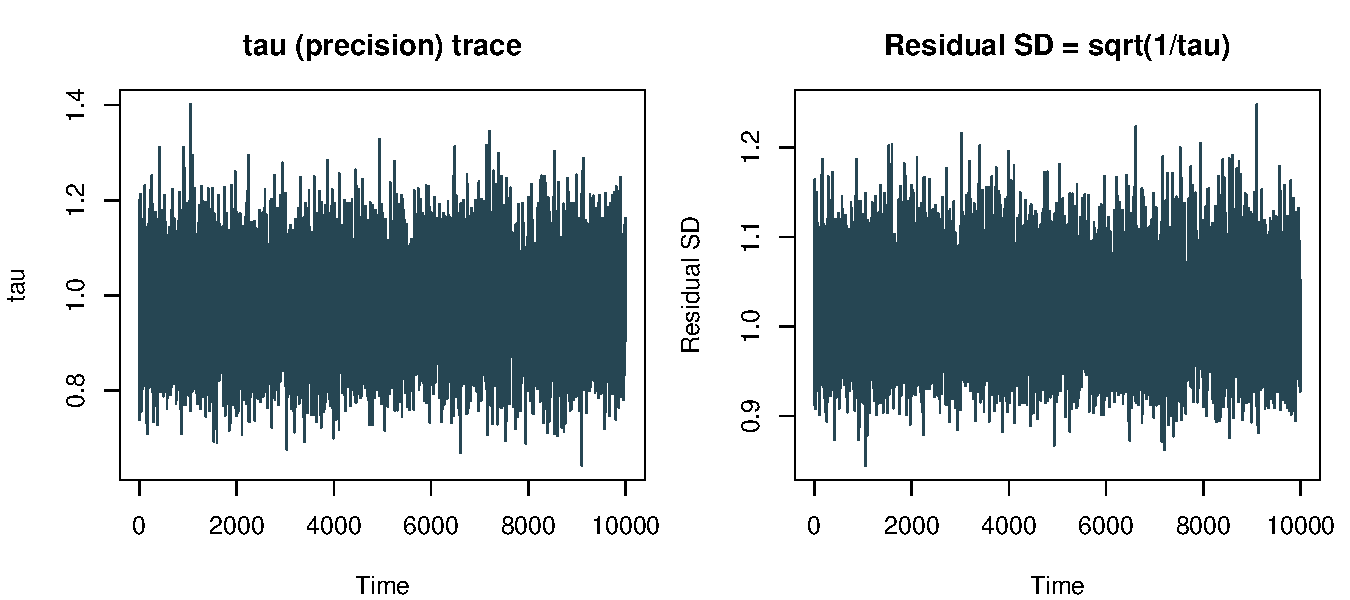
\includegraphics[width=0.8\textwidth]{03_trace_tau.pdf}
  \caption{Trace for the residual precision $\tau$ and the induced
           residual standard deviation $\sqrt{1/\tau}$.}
  \label{fig:trace-tau}
\end{figure}

\subsection*{D. Reproducibility}
All analysis code, raw data, construct scores, segment labels, and
figures are in the project repository
\href{https://github.com/AHMerrill/BNPL-final-project}{AHMerrill/BNPL-final-project}.
The analysis reproduces end-to-end by running, in order,
\texttt{R/01\_pca.R}, \texttt{R/00\_eda.R}, \texttt{R/02\_cluster.R},
and \texttt{R/03\_bayes\_hlm.R} from the repository root. Required
R packages: \texttt{readxl}, \texttt{mclust}, \texttt{mvtnorm},
\texttt{MCMCpack}, \texttt{lme4}.

\end{document}
